\chapter*{Annexes}

\section*{Terminaison anéchoïque}
\label{term_anecho}
La terminaison anéchoïque est constituée de fin tissu métallique résistif aucun viens s'ajouter une cavité de section variable qui crée une discontinuité de section. Afin de fixer cette dernière on procède au calcul du coefficient de réflexion du réseau sans aucun résonateurs (juste le tube). Le but est de voir quel est l'impacte de l'onde réfléchi par la sortie anéchoïque sur l'entrée du réseau. Après réglage, la courbe de réflexion figure~\ref{fig_term_anecho} est finalement obtenu.

\begin{figure}
\centering
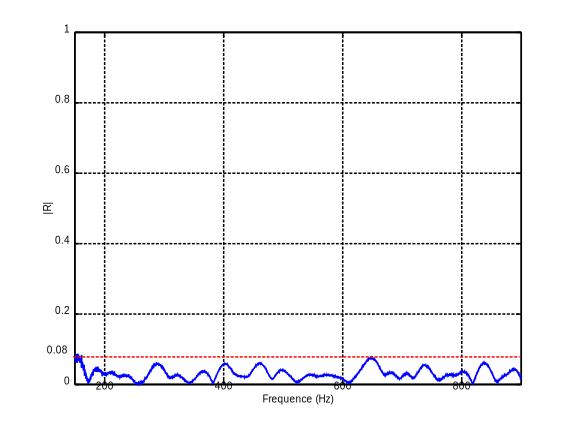
\includegraphics[scale=0.5]{./images_annexe/anecho.png}
\caption{\label{fig_term_anecho} Coefficient de réflexion pour le réseau sans résonateur avec une terminaison anéchoïque adaptée.}
\end{figure}

On constate que le coefficient de réflexion ne dépasse jamais 0.08 ce qui semble tout à fait acceptable afin de considérer la sortie comme anéchoïque dans le reste du projet.

\section*{Annexe 2: Paramètres du réseau étudié }
La liste des dimensions du réseau utilisé lors des expériences et des simulations est la suivante:
\begin{itemize}
\item Le guide a un rayon de $R_t = 2.5~cm$ et une épaisseur de $ep = 0.5~cm$.
\item Les résonateur sont composées de 2 tubes: le col de $R_n = 1~cm$ de rayon et $L_n = 2~cm$ de longueur, la cavité de $R_c = 2.15~cm$ de rayon et de longueur variable $L_c$. C'est cette dernière longueur qui permet de faire varier la fréquence de résonance du résonateur. 
\end{itemize}

\bigskip
Les corrections apportées aux cols des résonateurs sont les suivantes:
\begin{eqnarray*}
l_1 & = &  0.82 \left[ 1 - 1.35 \frac{R_n}{R_c} + 0.31 \left(\frac{R_n}{R_c} \right)^3  \right] R_n \\
l_2 & = &  0.82 \left[ 1 - 0.235 \frac{R_n}{R_t} - 1.32 \left( \frac{R_n}{R_t} \right)^2 +1.54 \left( \frac{R_n}{R_t}\right)^3 - 0.86 \left( \frac{R_n}{R_t}\right)^4  \right] R_n \\
L_{corr} & = &  l_1 + l_2
\end{eqnarray*}
